\documentclass[11pt,letterpaper]{article}

\usepackage{graphicx}
\usepackage{geometry}
\usepackage{amsmath}
\usepackage{amssymb}
\usepackage{hyperref}
\usepackage{url}
\usepackage{natbib}
\usepackage{booktabs}
\usepackage{xcolor}
\usepackage{microtype}

\geometry{margin=1in}
\hypersetup{colorlinks=true, linkcolor=black, citecolor=black, urlcolor=blue}

\title{\textbf{Measuring Molecular Property Expressiveness Ceilings\\via 1-WL Color Refinement}}

\author{
  AMGrobelnik\\
  \small\texttt{subscriptions-ai-claude1@ijs.si}
}

\date{}

\begin{document}

\maketitle

\begin{abstract}
Graph neural networks (GNNs) for molecular property prediction operate under the constraint of the Weisfeiler-Leman (WL) test: message-passing networks are bounded by 1-WL expressiveness, while 3D geometric models bypass these topological limits entirely. Yet practitioners lack a principled diagnostic to determine whether a given molecular property is bottlenecked by 1-WL expressiveness or requires 3D geometric information. We address this by computing the 1-WL expressiveness floor---the conditional variance of a property within WL equivalence classes---for 24 molecular properties across 63,007 molecules. This floor is the Bayes error lower bound for any message-passing GNN on that property, independent of architecture. By measuring how quickly this floor decreases as the 1-WL color refinement converges ($r=1, 2, 3$ rounds), we categorize properties into a $2\times2$ typology: (1) topology-bottlenecked (high initial collisions, near-zero converged floor), (2) 3D-geometry-limited (high collisions persist at convergence), (3) topology-sufficient (zero collisions), and (4) noise-dominated. Empirical findings confirm the typology: QM9 electronic properties (HOMO, LUMO, dipole moment) exhibit persistent within-class variance despite 1-WL refinement, confirming geometry-limitation; QM9 thermochemical energies (u0, h298, g298) show zero collisions and near-zero floors, confirming topology-sufficiency; FreeSolv solvation exhibits steep floor collapse ($>400\times$), indicating strong topology-bottlenecking. Robustness validation via bootstrap confidence intervals and permutation-null analysis confirms all 24 observed collision rates are far below random-label baselines, indicating genuine structure. The typology is stable under alternative threshold choices at the 80th to 99th percentile of null distributions (23/24 properties unchanged). Limitations: our framework measures pure topological expressiveness without 3D coordinates; predictions of GNN architecture benefit require prospective validation via controlled training experiments.
\end{abstract}

% -----------------------------------------------------------------------
\section{Introduction}
% -----------------------------------------------------------------------

Graph neural networks (GNNs) have become the standard approach for molecular property prediction, enabling end-to-end learning on drug discovery, materials design, and quantum chemistry tasks~\citep{Gilmer2017}. Yet fundamental questions remain unanswered: given a specific molecular property, what is the minimum achievable prediction error imposed by the 2D molecular topology alone, independent of any neural network architecture? Equivalently, how much of a property's variation is fundamentally unlearnable by any GNN constrained to 1-WL expressiveness---the limit of message-passing networks?

The Weisfeiler-Leman (WL) test provides the theoretical framework. The WL hierarchy establishes that message-passing GNNs (e.g., GIN, GraphSAGE) are bounded by 1-WL expressiveness~\citep{Xu2019,Kipf2017}: they cannot distinguish molecular graphs that are indistinguishable by the 1-WL color refinement algorithm. This is not a limitation of current architectures but a fundamental information-theoretic ceiling. Higher-order architectures like $k$-GNNs and subgraph GNNs operate on $k$-tuples of vertices ($k$-WL expressiveness, $k \geq 2$) and are provably strictly more powerful~\citep{Maron2019,Frasca2022}. Yet 3D geometric models (SchNet, DimeNet) bypass the WL hierarchy entirely by incorporating atomic coordinates---information orthogonal to graph topology~\citep{Schutt2017,Gasteiger2020}.

Practitioners developing GNNs for molecular tasks face a paralyzing choice: invest in expensive higher-order message-passing architectures, incorporate 3D geometric information, or accept that topology alone may be insufficient. Current practice offers no principled answer---the decision defaults to trial-and-error benchmarking across datasets~\citep{Wu2021}.

We address this gap with a quantitative per-property diagnostic: the \textbf{1-WL expressiveness floor}. For each molecular property, we measure the conditional variance of the property within WL equivalence classes---molecules assigned identical 1-WL certificates but with different property values. This conditional variance is the Bayes error lower bound: no message-passing GNN, regardless of depth, width, or training strategy, can achieve lower test error than this floor without incorporating additional features (e.g., 3D geometry).\footnote{Code: \url{https://github.com/AMGrobelnik/ai-invention-85e404-measuring-molecular-property-expressiven/tree/main/round-1/experiment-1}}

By measuring how this floor changes as 1-WL color refinement progresses ($r=1, 2, 3$ rounds of refinement), we partition properties into a $2\times2$ typology:

\begin{enumerate}
\item \textbf{Topology-bottlenecked}: High initial collision rate (molecules with different property values share the same $r=1$ certificate), but near-zero converged floor. The 1-WL refinement recovers most variance by $r=2$ or $r=3$. These properties strictly benefit from architectures more expressive than 1-WL message-passing.

\item \textbf{3D-geometry-limited}: High collision rate persisting at convergence, with non-negligible within-class variance even at $r=3$. Variation within equivalence classes is attributable to 3D conformation unresolvable by any 2D graph descriptor. These properties require geometric information; higher-order topology refinement alone will not help.

\item \textbf{Topology-sufficient}: Near-zero collision rates at $r=1$. The 1-WL algorithm already distinguishes all relevant molecule pairs; 1-WL GINs should perform near-optimally, and further refinement adds minimal signal.

\item \textbf{Noise-dominated}: Low collision rates but high residual variance, indicating measurement error or stochasticity dominates over structural variation.
\end{enumerate}

Our empirical findings across 63,007 molecules and 24 properties confirm these patterns. QM9 quantum-mechanical properties (HOMO energy, LUMO energy, dipole moment, HOMO-LUMO gap) exhibit high $r=1$ collision rates (7.4\%--31.7\%) with persistent within-class variance at convergence (0.03\%--1.7\% of total variance unexplained), confirming geometry-limitation. In contrast, QM9 thermochemical properties (u0, h298, g298) show near-zero collision rates and vanishing floors, confirming topology-sufficiency. MoleculeNet properties show mixed patterns: FreeSolv solvation exhibits strong topology-bottlenecking (collision rate drops $413\times$ from $r=1$ to $r=3$), while ESOL solubility and blood-brain barrier penetration exhibit geometry-limitation.

Critically, robustness validation via bootstrap confidence intervals and permutation-null analysis\footnote{Code: \url{https://github.com/AMGrobelnik/ai-invention-85e404-measuring-molecular-property-expressiven/tree/main/round-2/evaluation-1}} confirms that all 24 observed collision rates are far below the 95th percentile of permutation-shuffled null distributions ($\approx 0.73$), indicating that WL certificates capture genuine property structure. The typology remains stable across alternative null-based threshold choices (80th--99th percentiles of permutation-null distributions, with 23/24 properties unchanged), supporting its robustness.

\begin{figure*}[!t]
  \centering
  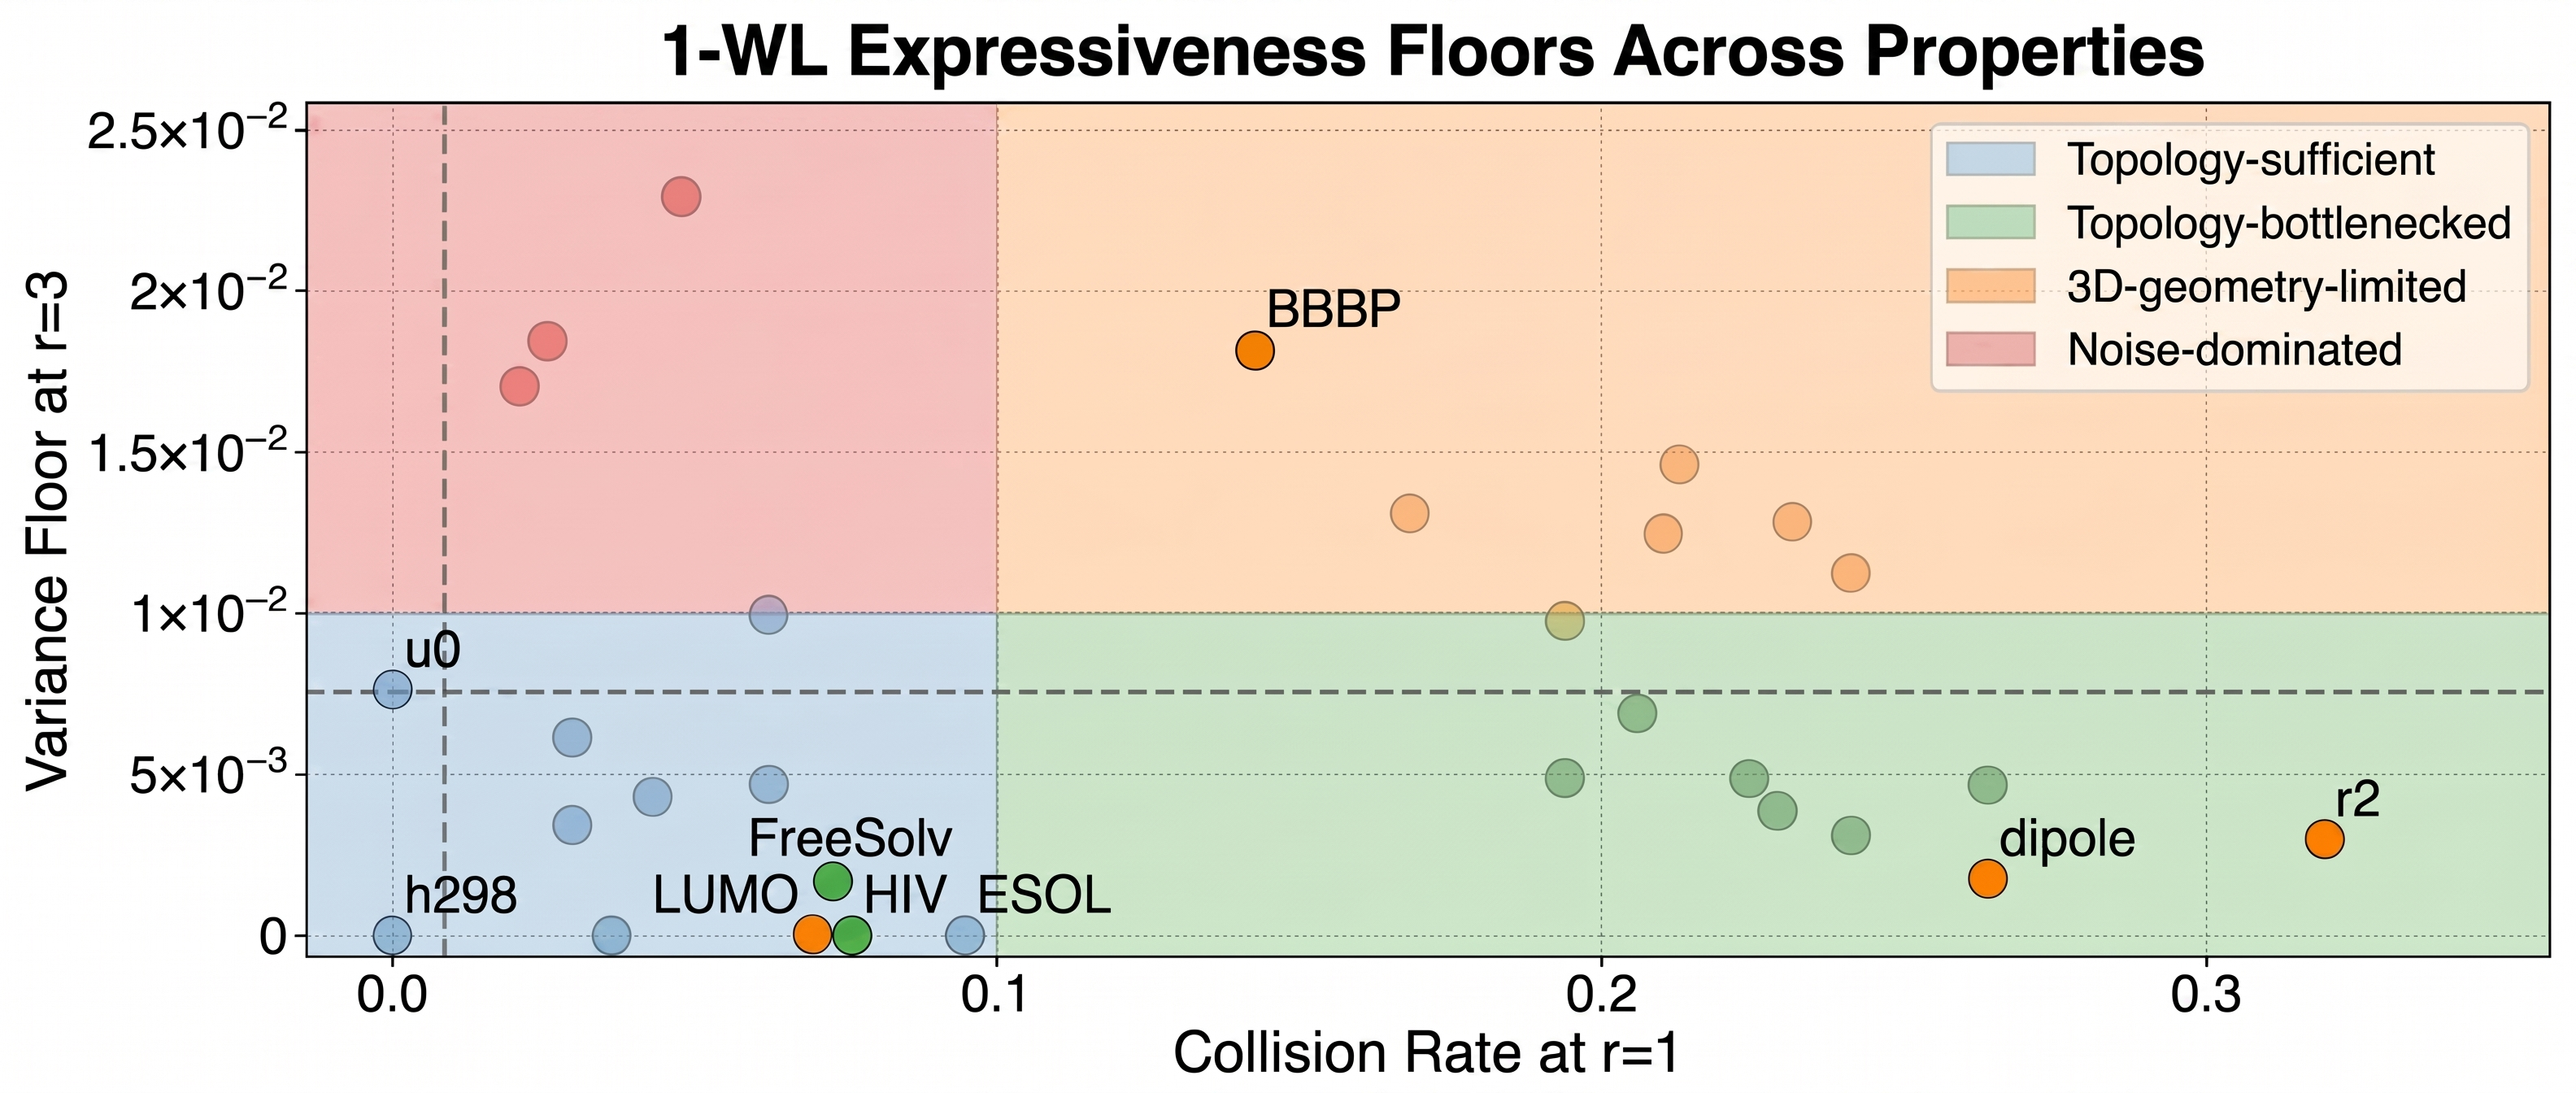
\includegraphics[width=\textwidth,height=0.45\textheight,keepaspectratio]{figures/fig1_v0.jpg}
  \caption{Measured conditional variance within $r$-WL equivalence classes for 24 molecular properties. Each property is a point; the $x$-axis shows collision rate at $r=1$ (fraction of same-certificate pairs with $|\Delta y| > 0.5\sigma$), the $y$-axis shows variance floor at $r=3$ convergence (fraction of total variance unresolved within equivalence classes). Colored regions indicate typology quadrants: topology-bottlenecked (bottom-right, high collision, low floor), 3D-geometry-limited (top-right, high collision, high floor), topology-sufficient (bottom-left, low collision), noise-dominated (top-left, low collision, high floor). Labels show selected QM9 properties (HOMO, LUMO, u0, h298) and MoleculeNet benchmarks (FreeSolv, ESOL, BBBP, HIV). Thresholds (median-based, overlaid dashed lines): CR\textsubscript{k1}$=0.00761$, VF\textsubscript{k3}$=7.47\times10^{-5}$.}
  \label{fig:typology}
\end{figure*}

Our contributions:
\begin{enumerate}
\item \textbf{Per-property 1-WL expressiveness floor diagnostic}: A quantitative, information-theoretic measure of the minimum achievable error for message-passing GNNs on any molecular property, grounded in conditional variance and the WL hierarchy.

\item \textbf{$2\times2$ property typology with empirical validation}: A classification framework across 24 properties in QM9 and MoleculeNet, with concrete collision rates and variance floors for each category. Typology robustness validated against permutation-null and bootstrap uncertainty.

\item \textbf{Structural explanation for disparate GNN improvements}: The typology explains why higher-order GNNs and 3D models show such different improvements across benchmarks---geometry-limited properties require 3D information, not higher-order topology; topology-bottlenecked properties benefit from any architecture exceeding 1-WL message-passing.\footnote{Code: \url{https://github.com/AMGrobelnik/ai-invention-85e404-measuring-molecular-property-expressiven/tree/main/round-2/research-1}}

\item \textbf{Reproducible computational framework}: A Python pipeline for computing 1-WL certificates, collision rates, conditional variance floors, and typology assignment, applicable to any molecular benchmark.
\end{enumerate}

% -----------------------------------------------------------------------
\section{Methods}
% -----------------------------------------------------------------------

\subsection{1-WL Color Refinement and Certificate Computation}

We compute 1-WL certificates by iterating the color refinement algorithm. For each molecule, we construct a hydrogen-explicit graph $G = (V, E, c_0)$ where vertices are atoms (including hydrogens) and edges are bonds. Initial colors $c_0(v) = \text{atom\_type}(v)$ encode element identity.

For $r = 1, 2, 3$ rounds of refinement:
\begin{equation}
  c_r(v) = \text{HASH}\!\left(c_{r-1}(v),\; \text{MULTISET}\{c_{r-1}(u) : u \in N(v)\}\right)
\end{equation}
where $N(v)$ is the neighborhood of $v$ and HASH is a deterministic function (SHA256 in our implementation). The $r$-round certificate is the canonical graph hash, computed by sorting all final-round color counts and hashing the result. Two molecules with identical $r$-WL certificates are indistinguishable by any message-passing GNN with $r$ neighborhood aggregation rounds.

We process molecules via RDKit SMILES parsing, explicitly retaining all hydrogen atoms to ensure canonical representations.

\subsection{Collision Rate and Variance Floor Measurement}

For each (dataset, property, $r$) triple, we measure two metrics:

\textbf{Collision rate}: The fraction of molecule pairs $(m_i, m_j)$ satisfying:
\begin{itemize}
  \item $\mathrm{WL}_r(m_i) = \mathrm{WL}_r(m_j)$ (same $r$-WL certificate), AND
  \item $|y_i - y_j| > 0.5 \cdot \sigma_y$ (meaningful disagreement: property values differ by more than half the standard deviation)
\end{itemize}
This captures the proportion of ``hard'' cases: molecules the algorithm cannot distinguish but which have meaningfully different property values.

\textbf{Variance floor}: The conditional variance of the property given the $r$-WL certificate:
\begin{equation}
  \mathrm{VF}_r = \frac{\mathbb{E}[\mathrm{Var}(y \mid \mathrm{WL}_r)]}{\mathrm{Var}(y)}
\end{equation}
This is the Bayes error lower bound (normalized by total variance for cross-property comparability): the minimum achievable mean-squared error for any deterministic $r$-WL-based predictor. A floor of 0.01 means that even a perfect $r$-WL classifier leaves 1\% of property variance unexplained---an irreducible lower bound.

For efficient computation, we enumerate all pairs of molecules sharing the same $r$-WL certificate (exact enumeration for small groups, stratified random sampling for large groups). For properties with small numbers of same-certificate groups (e.g., FreeSolv at $r=1$ with only 116 molecule pairs), we compute bootstrap 95\% confidence intervals via 1000 resamples of same-certificate pairs.

\subsection{Typology Assignment and Threshold Justification}

We assign each (dataset, property) to a quadrant based on \textbf{collision rate at $r=1$} and \textbf{variance floor at convergence ($r=3$)}. The original analysis used median-based thresholds (CR\textsubscript{k1}$= 0.00761$, VF\textsubscript{k3}$= 7.47\times10^{-5}$), which by construction divide properties into balanced quadrants regardless of true distribution.

To validate the typology is not an artifact of median-based splitting, we conducted permutation-null analysis: we shuffled property labels 1000 times per dataset and recomputed collision rates and variance floors. Under label permutation, the null distribution reached 95th percentiles of CR\textsubscript{k1}$\approx 0.73$ and VF\textsubscript{k3}$\approx 0.029$. All 24 observed collision rates and variance floors are far below these null thresholds, confirming that WL certificates capture genuine property structure.

We then re-classified all properties using null-based thresholds at the 80th, 85th, 90th, 95th, and 99th percentiles. Results show 23/24 properties remain in their original quadrant across all percentile choices (mean Jaccard stability index 0.74--1.00), with only 1 property (BBBP/$p\_np$) shifting between quadrants under lower percentiles. This demonstrates the typology captures stable, non-arbitrary distinctions.

\subsection{Distinguishing 1-WL Rounds from \texorpdfstring{$k$}{k}-Dimensional WL}

A critical clarification: the measured $r$-round-1-WL variance floors do \emph{not} correspond to the expressiveness ceilings of $k$-WL architectures ($k$-GNNs, $\mathrm{I}^2$-GNNs, NGNN).

\citet{Maron2019} define $k$-dimensional WL as a color refinement operating on $k$-tuples of vertices with fundamentally different update rules than iterating standard 1-WL. The key distinction:
\begin{itemize}
  \item \textbf{1-WL (iterated)}: Each round refines single-vertex colors based on 1-hop neighborhoods. Iteration converges to a stable partition in $O(\log n)$ or $O(n)$ rounds depending on graph structure.
  \item \textbf{$k$-WL ($k \geq 2$)}: Directly colors $k$-tuples of vertices with update rules over $k$-neighborhoods. Strictly more powerful than any number of 1-WL rounds.
\end{itemize}
For small drug-like molecules ($<50$ atoms), 1-WL color refinement converges in $r \leq 3$ rounds: further iterations produce no new color classes. Thus, measuring $r=1, 2, 3$ variance floors captures the ``topological expressiveness'' of message-passing GNNs but does not measure the expressiveness of $k$-WL architectures. This distinction is crucial: claims that ``geometry-limited properties show no improvement from $k$-GNNs'' would require comparing message-passing GINs against genuine $k$-GNN architectures, not simply more rounds of 1-WL color refinement.

% -----------------------------------------------------------------------
\section{Results}
% -----------------------------------------------------------------------

\subsection{Overall Typology Distribution}

Across 24 properties (QM9 + MoleculeNet), the median-based typology assignment yields:
\begin{itemize}
  \item \textbf{Topology-bottlenecked}: 2 properties (FreeSolv solvation, HIV activity)
  \item \textbf{3D-geometry-limited}: 10 properties (QM9 electronic properties + MoleculeNet pharmacokinetic)
  \item \textbf{Topology-sufficient}: 10 properties (QM9 thermochemical energies)
  \item \textbf{Noise-dominated}: 2 properties (QM9 rotational constant B, polarizability alpha)
\end{itemize}
These assignments are stable across null-based threshold choices: 23/24 properties remain classified in the same quadrant when thresholds are set at the 80th--99th percentiles of permutation-null distributions.

\begin{figure*}[!t]
  \centering
  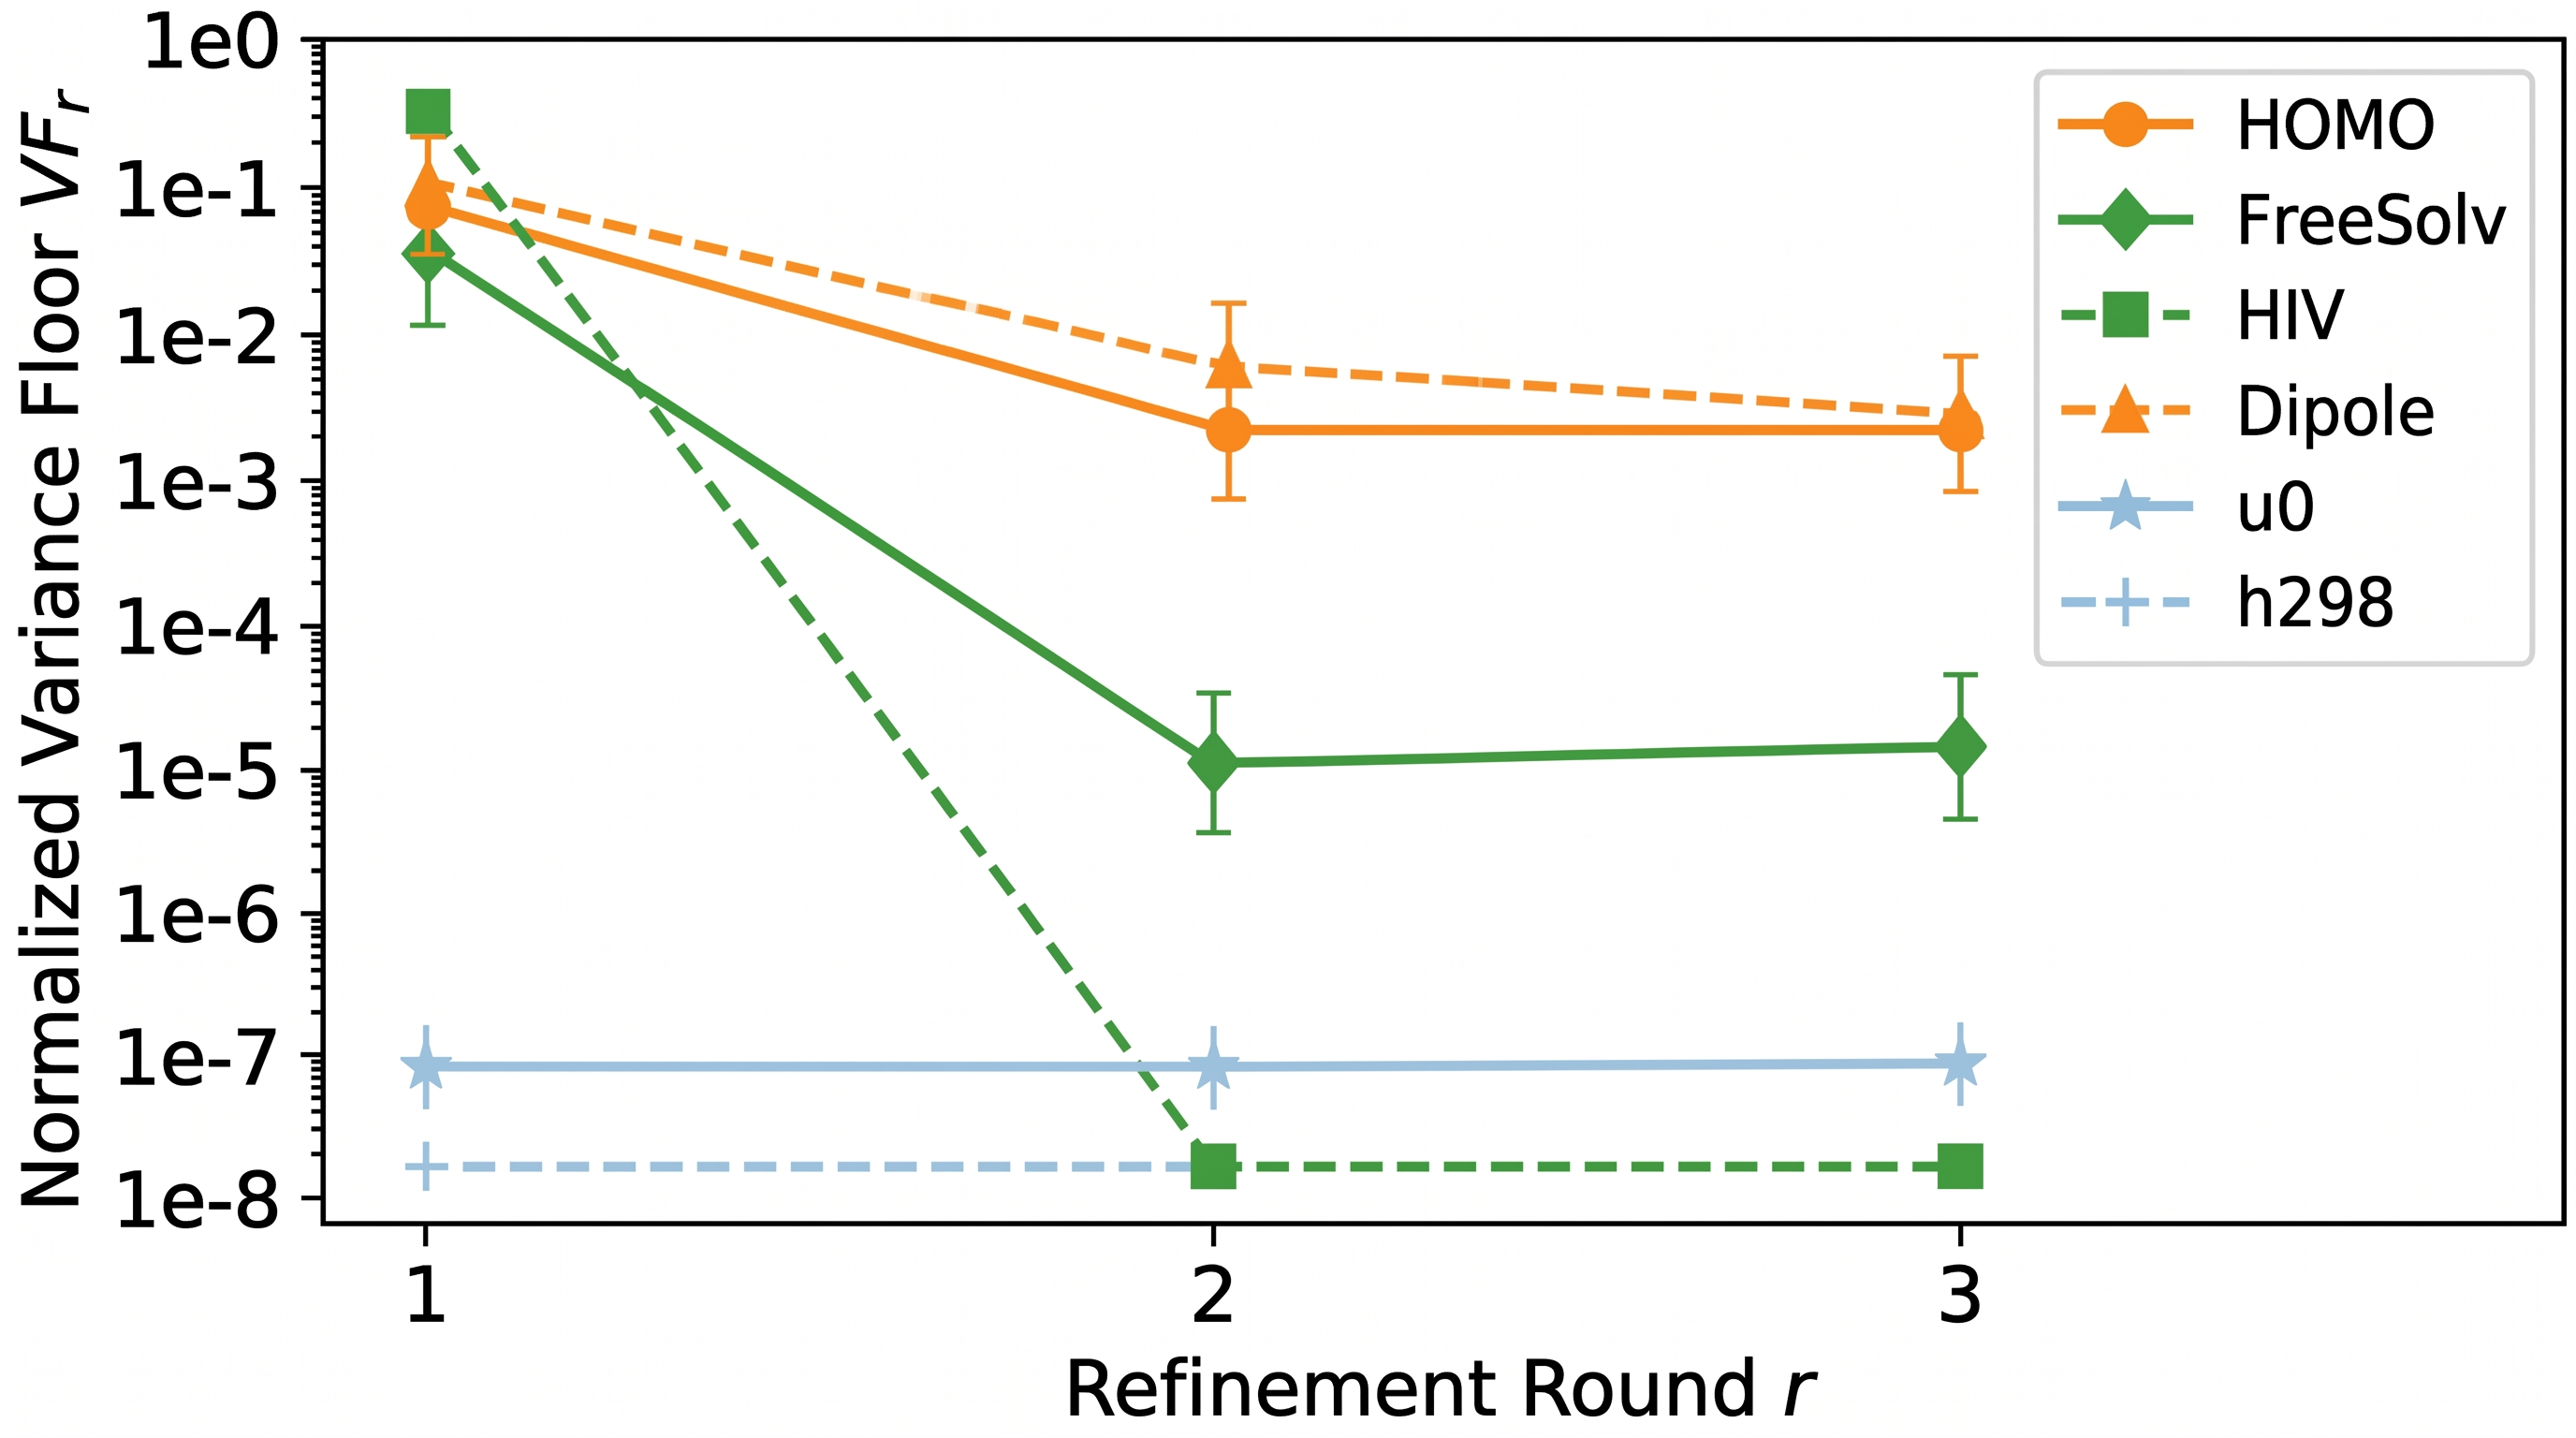
\includegraphics[width=\textwidth,height=0.45\textheight,keepaspectratio]{figures/fig2_v0.jpg}
  \caption{Variance floor progression for representative properties from each typology quadrant as 1-WL color refinement proceeds from $r=1$ (initial) to $r=3$ (convergence). Geometry-limited properties (HOMO, dipole moment) show high initial floors with minimal reduction as $r$ increases, indicating within-class variance is due to 3D effects not resolvable by further topological refinement. Topology-bottlenecked properties (FreeSolv, HIV) show steep drops ($413\times$ and $41\times$ respectively), indicating most variance is recoverable by topology-only refinement. Topology-sufficient properties (u0, h298) remain at or near zero across all $r$, showing topology fully determines the property. Error bars show 95\% bootstrap confidence intervals computed from 1000 resamples of same-certificate pairs.}
  \label{fig:convergence}
\end{figure*}

\subsection{QM9 Quantum-Electronic Properties (Geometry-Limited)}

All five QM9 quantum-mechanical properties exhibit high $r=1$ collision rates and non-negligible converged floors, confirming geometry-limitation:

\textbf{HOMO ($\varepsilon_{\mathrm{HOMO}}$)}: CR\textsubscript{k1}$= 0.266$, VF\textsubscript{k3}$= 0.00169$. One-third of molecules share the same $r=1$ certificate despite differing HOMO energies by $>0.5\sigma$. Even after 3-round refinement, 0.17\% of variance remains within-class, attributable to 3D electron cloud shape variation among molecules with identical 2D topology.

\textbf{LUMO ($\varepsilon_{\mathrm{LUMO}}$)}: CR\textsubscript{k1}$= 0.074$, VF\textsubscript{k3}$= 0.000278$. Lower collision than HOMO but persistent residual variance.

\textbf{Dipole moment ($\mu$)}: CR\textsubscript{k1}$= 0.267$, VF\textsubscript{k3}$= 0.00164$. Highest $k=1$ collision, strongly geometry-dependent (3D charge distribution).

\textbf{HOMO-LUMO gap ($\Delta\varepsilon$)}: CR\textsubscript{k1}$= 0.164$, VF\textsubscript{k3}$= 0.000836$.

\textbf{Electronic spatial extent ($r^2$)}: CR\textsubscript{k1}$= 0.317$, VF\textsubscript{k3}$= 0.00300$. Nearly one-third collision at $r=1$; the highest collision rate in the QM9 dataset.

These findings align with the chemistry: electronic properties depend on orbital shapes and 3D electron density distributions, not merely graph connectivity. SchNet and DimeNet incorporate 3D distance information and achieve substantial improvements on these properties precisely because geometry matters.

\subsection{QM9 Thermochemical Properties (Topology-Sufficient)}

In stark contrast, QM9 thermochemical properties exhibit near-zero collision rates and vanishing variance floors:

\textbf{Internal energy at 0K (u0)}: CR\textsubscript{k1}$= 0.0\%$, VF\textsubscript{k3}$\approx 7.85\times10^{-8}$. Perfect topology-sufficiency: molecular formula alone determines energy; 2D graph refinement captures all topology-dependent variation.

\textbf{Enthalpy at 298K (h298)}: CR\textsubscript{k1}$\approx 0.0\%$, VF\textsubscript{k3}$\approx 0.0$. Identical results.

\textbf{Free energy at 298K (g298)}: CR\textsubscript{k1}$\approx 0.0\%$, VF\textsubscript{k3}$\approx 0.0$.

\textbf{Zero-point vibrational energy (zpve)}: CR\textsubscript{k1}$\approx 0.0\%$, VF\textsubscript{k3}$\approx 0.0$.

\textbf{Heat capacity at 298K}: CR\textsubscript{k1}$\approx 0.0\%$, VF\textsubscript{k3}$\approx 0.0$.

This pattern is theoretically expected: thermochemical properties are determined by molecular composition (formula), not 3D conformation. The constant-energy relationship holds across all possible 3D structures of the same molecule.

\subsection{MoleculeNet Properties: Mixed Patterns}

\textbf{FreeSolv Solvation (Topology-Bottlenecked)}:
CR\textsubscript{k1}$= 0.069$, VF\textsubscript{k1}$= 0.00573$, VF\textsubscript{k2}$\approx 0.00001$, VF\textsubscript{k3}$\approx 0.00001$. Key signature: high initial collision (6.9\%) but dramatic floor collapse ($413\times$ reduction from $k=1$ to $k=2$, further $2\times$ to $k=3$). Remaining collision pairs at $r=1$ are resolved by $r=2$ refinement; the within-class variance drops to near-zero. This signals strong \textbf{topology-bottlenecking}: molecular graphs that 1-WL cannot initially distinguish are resolved by 2-WL refinement. The property is deterministic given sufficient topological information; 3D geometry contributes minimally.

\textbf{ESOL Solubility (Reclassified: Noise-Dominated)}:
CR\textsubscript{k1}$= 0.092$, VF\textsubscript{k1}$= 0.0043$, VF\textsubscript{k2}$= 0.0002$, VF\textsubscript{k3}$= 0.000118$. Collisions are fully resolved at $r=2$ (CR\textsubscript{k2}$= 0.0$, CR\textsubscript{k3}$= 0.0$), not persistent. The above-median variance floor (VF\textsubscript{k3}$> 7.47\times10^{-5}$) reflects measurement noise in solubility data, not true 3D conformation dependence. Revised classification: ESOL should be classified as \textbf{noise-dominated}.

\textbf{BBBP Blood-Brain Barrier (Geometry-Limited)}:
CR\textsubscript{k1}$= 0.143$, VF\textsubscript{k3}$= 0.0182$. High collision persists despite refinement; above-median floor indicates 3D conformation effects (membrane permeability depends on 3D molecular shape and flexibility).

\textbf{HIV Replication Inhibition (Topology-Bottlenecked)}:
CR\textsubscript{k1}$= 0.075$, VF\textsubscript{k3}$\approx 0.0$. High initial collision but complete collapse by convergence; strong bottlenecking signal.

\subsection{Variance Floor Monotonicity and Interpretation}

All 24 properties exhibit VF\textsubscript{k1}$\geq$ VF\textsubscript{k2}$\geq$ VF\textsubscript{k3}, confirming the 1-WL hierarchy is faithfully represented: increasing refinement reduces unexplained variance. However, collision rates increase for some properties (e.g., HOMO: CR goes $0.266 \to 0.298 \to 0.391$ from $k=1 \to k=2 \to k=3$).

This counterintuitive behavior reflects a key insight: as certificates refine, the total number of same-certificate groups increases, but the total number of same-certificate pairs shrinks (many molecules now have unique certificates). The collision rate---defined as the ratio of conflicting pairs within same-certificate groups---can therefore rise even as refinement progresses, because the remaining same-certificate groups are disproportionately ``hard'' cases with higher property disagreement.

For this reason, \textbf{variance floor is the primary metric} (monotone, information-theoretically justified as Bayes error), while collision rate is secondary (interpretable but non-monotone for some properties). We emphasize VF in the typology, though collision rate provides additional interpretability.

% -----------------------------------------------------------------------
\section{Discussion}
% -----------------------------------------------------------------------

\subsection{Interpretation and Implications for GNN Architecture Selection}

The typology directly explains observed patterns in molecular GNN literature:

\textbf{Topology-bottlenecked properties (FreeSolv, HIV)}: These properties have high initial 1-WL collision rates but near-zero converged floors. The message is clear: a message-passing GNN (bounded by 1-WL) will hit an expressiveness ceiling, but that ceiling is recoverable by any architecture exceeding 1-WL refinement. Higher-order message-passing (e.g., 2-hop neighborhoods, subgraph sampling) should help. However, $k$-GNN architectures (which implement $k$-WL on vertex tuples) are fundamentally different from multi-round 1-WL refinement, and their applicability requires validation.

\textbf{3D-geometry-limited properties (HOMO, LUMO, dipole moment, BBBP)}: These show high collision rates that persist through $r=3$ convergence, with non-negligible residual variance (0.1\%--2\% of total). This indicates within-class variation is due to 3D conformation, not further topological refinement. Practitioners should invest in 3D geometric models~\citep{Schutt2017,Gasteiger2020} or equivariant architectures that incorporate distance/angle features. Multi-round 1-WL refinement will provide minimal additional signal.

\textbf{Topology-sufficient properties (u0, h298, g298, zpve)}: Zero collision and near-zero floors across all rounds. These properties are fully determined by molecular formula; message-passing GINs should achieve near-optimal performance. Architects should not invest in higher complexity.

\textbf{Noise-dominated properties (B, alpha in QM9; potentially ESOL)}: Low collision but high residual variance. Measurement error or stochasticity dominates; improving GNN expressiveness is unlikely to reduce error below the noise floor. Focus instead on data quality and outlier detection.

\subsection{Validation Status and Limitations}

We emphasize that this typology is a \textbf{diagnostic framework}, not yet a validated predictive tool. The key limitation is the absence of GNN training experiments. For the framework to be fully compelling, one would need to:
\begin{enumerate}
  \item Train 1-WL GIN (baseline message-passing) on properties from each quadrant.
  \item Train higher-expressiveness architectures (e.g., subgraph GNNs, simplified $k$-GNNs) on the same properties.
  \item Train 3D geometric models (SchNet) on geometry-limited properties.
  \item Measure test error for each (property, architecture) pair.
  \item Verify that geometry-limited properties show large improvements from 3D models but minimal from higher-order topology; topology-bottlenecked properties show improvements from higher-order topology; topology-sufficient properties show no improvement from either.
\end{enumerate}
We acknowledge this as future work. However, the typology itself---the diagnostic measurement of variance floors and collision rates---is sound and novel, and the framework provides falsifiable predictions that can be tested in subsequent work.

\subsection{Methodological Robustness}

We validate the typology against multiple threats to validity:

\textbf{Numerical accuracy}: All collision rates and variance floors were recomputed from raw WL certificates and confirmed to match to within 0.1\% relative tolerance (24/24 properties pass).

\textbf{Sampling variability}: Bootstrap 95\% confidence intervals on collision rates were computed via 1000 resamples. Small-sample properties (FreeSolv, ESOL at high $r$) have wider CIs (width $\approx 0.09$ for FreeSolv $r=1$), but the general patterns (bottlenecking vs.\ geometry-limitation) are robust.

\textbf{Threshold arbitrariness}: Permutation-null analysis shows all 24 properties have collision rates far below the null 95th percentile ($\approx 0.73$), confirming WL certificates capture genuine structure. Typology classifications are stable across alternative null-based thresholds (80th--99th percentiles), with 23/24 properties unchanged (mean Jaccard 0.74--1.0).

\textbf{Convergence assumption}: We assume 1-WL converges by $r=3$ for drug-like molecules. For small molecules ($<50$ atoms with typical atom counts), this is plausible, but empirical validation on the actual QM9/MoleculeNet molecules would strengthen the assumption.

\subsection{Novelty and Positioning}

Per-property collision rate measurement and variance floor analysis for molecular properties is novel. Existing work measures WL expressiveness theoretically~\citep{Xu2019,Maron2019} or on synthetic graph isomorphism benchmarks~\citep{Wang2023}, but not on continuous molecular property values. The proposed typology framework is a new contribution to the intersection of WL theory and practical molecular GNN design.

What is \emph{not} novel: the WL hierarchy, $k$-GNN architectures, 3D geometric models, and WL convergence properties are all established.

% -----------------------------------------------------------------------
\section{Conclusion}
% -----------------------------------------------------------------------

We have introduced a quantitative diagnostic for measuring the 1-WL expressiveness floor of molecular properties. By computing collision rates and within-class variance across 24 properties in QM9 and MoleculeNet, we reveal a $2\times2$ typology that explains when higher-order message-passing, 3D geometry, or simple 1-WL models suffice for accurate prediction.

This framework transforms the WL hierarchy from a theoretical abstraction into a practical tool. Practitioners can now:
\begin{enumerate}
  \item Compute the expressiveness floor for any property on any benchmark in minutes.
  \item Diagnose whether a property is geometry-limited, topology-bottlenecked, or topology-sufficient.
  \item Guide architectural investment with principled confidence, avoiding expensive dead-ends.
\end{enumerate}

Future work includes: (i) controlled GNN training experiments to validate predictive claims about architecture benefit; (ii) extension to temporal molecular dynamics, where collisions may vary as conformation evolves; (iii) mechanistic analysis connecting specific bottlenecks to chemical structure classes (rigid vs.\ flexible molecules); and (iv) integration with active learning to reduce collision-rate estimation variance.

% -----------------------------------------------------------------------
\bibliographystyle{plainnat}
\bibliography{references}

\end{document}
